% ============================================================
%  ARCP Topology — Reference Document (Paper 1)
%  Student: Vignesh | Supervisor: Prof. Mouli
%  Source: De Doncker & Lyons, IEEE IAS 1990
%  Figures stored in: figures/
%  Naming convention: P1_Fig[N]_[description].png
%  Current figures available: P1_Fig5, P1_Fig7a--g
% ============================================================
\documentclass[12pt, a4paper]{article}

% ---- core packages ----
\usepackage[utf8]{inputenc}
\usepackage[T1]{fontenc}
\usepackage{amsmath, amssymb, amsthm}
\usepackage{bm}
\usepackage{siunitx}

% ---- figures ----
\usepackage{graphicx}
\graphicspath{{figures/}}           % all PNGs live here
\usepackage{float}
\usepackage{caption}
\usepackage{subcaption}

% ---- layout ----
\usepackage[a4paper, top=2.5cm, bottom=2.5cm, left=3cm, right=2.8cm]{geometry}
\usepackage{parskip}
\setlength{\parskip}{6pt}
\setlength{\parindent}{0pt}

% ---- hyperlinks ----
\usepackage[colorlinks=true, linkcolor=blue!60!black, citecolor=blue!50!black]{hyperref}

% ---- styled boxes ----
\usepackage{tcolorbox}
\tcbuselibrary{skins, breakable}

% ---- tables ----
\usepackage{booktabs}
\usepackage{array}
\usepackage{longtable}

% ---- section formatting ----
\usepackage{titlesec}
\usepackage{xcolor}
\definecolor{arcpblue}{RGB}{15, 58, 112}
\definecolor{arcporange}{RGB}{185, 72, 10}
\definecolor{arcpgreen}{RGB}{10, 100, 42}
\definecolor{arcpred}{RGB}{170, 25, 25}
\definecolor{lightblue}{RGB}{216, 232, 252}
\definecolor{lightorange}{RGB}{255, 244, 220}
\definecolor{lightgreen}{RGB}{216, 247, 228}
\definecolor{lightred}{RGB}{255, 228, 228}
\definecolor{lightgray}{RGB}{245, 245, 245}

\titleformat{\section}{\large\bfseries\color{arcpblue}}{{\thesection.}}{0.5em}{}
            [\vspace{-4pt}\rule{\textwidth}{0.5pt}]
\titleformat{\subsection}{\normalsize\bfseries\color{arcpblue!80!black}}{{\thesubsection}}{0.5em}{}

% ---- tcolorbox styles ----
\newtcolorbox{circuitbox}[1][Circuit Description]{
    colback=lightblue, colframe=arcpblue, coltitle=white,
    fonttitle=\bfseries\small, title=#1,
    breakable, enhanced, left=4pt, right=4pt, top=4pt, bottom=4pt}

\newtcolorbox{statebox}[1][State Variables \& Parameters]{
    colback=lightorange, colframe=arcporange, coltitle=white,
    fonttitle=\bfseries\small, title=#1,
    breakable, enhanced, left=4pt, right=4pt, top=4pt, bottom=4pt}

\newtcolorbox{eqnbox}[1][Governing Equations]{
    colback=lightgreen, colframe=arcpgreen, coltitle=white,
    fonttitle=\bfseries\small, title=#1,
    breakable, enhanced, left=4pt, right=4pt, top=4pt, bottom=4pt}

\newtcolorbox{physbox}[1][Physical Interpretation]{
    colback=lightgray, colframe=gray!60, coltitle=white,
    fonttitle=\bfseries\small, title=#1,
    breakable, enhanced, left=4pt, right=4pt, top=4pt, bottom=4pt}

\newtcolorbox{warningbox}[1][Watch Out]{
    colback=lightred, colframe=arcpred, coltitle=white,
    fonttitle=\bfseries\small, title=#1,
    breakable, enhanced, left=4pt, right=4pt, top=4pt, bottom=4pt}

% ---- custom commands ----
\newcommand{\Vdc}{V_{dc}}
\newcommand{\vf}{v_f}
\newcommand{\ir}{i_r}
\newcommand{\IL}{I_L}
\newcommand{\Lr}{L_r}
\newcommand{\Cr}{C_r}
\newcommand{\omegar}{\omega_r}
\newcommand{\Zr}{Z_r}
\newcommand{\Vc}{V_{C1}}
\newcommand{\figref}[1]{Figure~\ref{#1}}

% ---- figure entry macro ----
% Usage: \figentry{label}{filename}{caption}{width}
\newcommand{\figentry}[4]{%
    \begin{figure}[H]
        \centering
        \includegraphics[width=#4\textwidth]{#2}
        \caption{#3}
        \label{#1}
    \end{figure}%
}

% ============================================================
\title{\textbf{Auxiliary Resonant Commutated Pole (ARCP) Converter}\\[4pt]
       \large Paper 1 — Circuit Diagrams, State Variables,\\
       \large Governing Equations, and Physical Interpretations\\[4pt]
       \normalsize De Doncker \& Lyons, IEEE IAS 1990}
\author{Vignesh\\[4pt]
        \small Supervised by: Prof.\ Mouli}
\date{\today}
% ============================================================

\begin{document}
\maketitle
\tableofcontents
\clearpage

% ============================================================
\section{How to Use This Document}
% ============================================================

Each figure section follows this standard four-block structure:

\begin{enumerate}
    \item \textbf{Figure} — the extracted PNG from the paper
    \item \textbf{Circuit Description} (blue box) — what components are present
          and how they are connected
    \item \textbf{State Variables \& Parameters} (orange box) — every symbol
          that appears in the figure, with units and typical values
    \item \textbf{Governing Equations} (green box) — all equations that apply
          to this circuit state, derived from first principles
    \item \textbf{Physical Interpretation} (gray box) — what the figure
          \emph{means}: energy flow, ZVS conditions, design trade-offs
\end{enumerate}

All figures are from: De Doncker \& Lyons,
\textit{The Auxiliary Resonant Commutated Pole Converter},
IEEE IAS Annual Meeting, 1990.

% ============================================================
\section{The ARCP Pole Leg — P1 Fig.\,5}
\label{sec:P1Fig5}
% ============================================================

\figentry{fig:P1Fig5}{P1_Fig5_ARCP_pole_leg.png}
         {The Auxiliary Resonant Commutated Pole (ARCP) single phase leg.
          Source: De Doncker \& Lyons, IEEE IAS 1990, p.\,3.}{0.75}

\begin{circuitbox}[Circuit Description — P1 Fig.\,5]
The ARCP pole leg consists of:
\begin{itemize}
    \item \textbf{DC bus}: split into two equal halves by two $2C_{dc}$
          capacitors, creating a midpoint rail at $\Vdc/2$
    \item \textbf{Main upper device}: $S_1$ (IGBT) with anti-parallel diode
          $D_1$; snubber capacitor $\Cr/2$ across $S_1$
    \item \textbf{Main lower device}: $S_2$ (IGBT) with anti-parallel diode
          $D_2$; snubber capacitor $\Cr/2$ across $S_2$
    \item \textbf{Pole node}: the junction of $S_1$ and $S_2$; voltage $\vf$
          swings between 0 and $\Vdc$ during commutation
    \item \textbf{Auxiliary switches}: $A_1$ and $A_2$ are back-to-back
          bidirectional switches (p-channel MCTs) connected between the
          \emph{DC bus midpoint} and the resonant inductor $\Lr$
    \item \textbf{Resonant inductor}: $\Lr$ connects from the $A_1$/$A_2$
          pair to the pole node; carries auxiliary current $\ir$
    \item \textbf{Load}: filter inductor $L_F$ and load current $I_F$ at
          the pole node; $V_F$ is the filtered output voltage
\end{itemize}
The auxiliary branch ($A_1$--$A_2$--$\Lr$) is \emph{only active during
commutation}. At steady state $\ir = 0$.
\end{circuitbox}

\begin{statebox}
\renewcommand{\arraystretch}{1.3}
\begin{tabular}{p{0.12\linewidth} p{0.32\linewidth} p{0.46\linewidth}}
\toprule
\textbf{Symbol} & \textbf{Quantity} & \textbf{Role} \\
\midrule
$\vf$      & Pole-node voltage           & Primary state variable; swings 0 to $\Vdc$ during commutation \\
$\ir$      & Auxiliary inductor current  & Secondary state variable; drives the $\Cr$ swing \\
$\IL$      & Load current (quasi-static) & Treated as constant disturbance during commutation. Note: labeled $I_F$ in Fig.\,5 but written $I_L$ in paper text — same quantity \\
$\Vdc$     & DC bus voltage              & Forcing potential across the pole \\
$\Lr$      & Auxiliary inductance        & Sets boost ramp rate and resonant frequency \\
$\Cr$      & Snubber capacitance         & Sets resonant frequency and commutation speed \\
$A_1, A_2$ & Auxiliary switches (MCTs)   & Fire for $T_\text{boost}$ duration only; silent otherwise \\
\bottomrule
\end{tabular}
\end{statebox}

\begin{eqnbox}
\textbf{Starting point — KCL and KVL during the resonant swing (Phase\,2 only):}
\begin{align}
    \frac{d\vf}{dt} &= \frac{\ir - \IL}{\Cr}       \label{eq:dvf_dt} \\[4pt]
    \frac{d\ir}{dt} &= \frac{\Vdc/2 - \vf}{\Lr}    \label{eq:dir_dt}
\end{align}

\medskip
\textbf{Step 1 — Eliminate $\ir$: differentiate \eqref{eq:dvf_dt}, substitute \eqref{eq:dir_dt}.}

Differentiate both sides of \eqref{eq:dvf_dt} with respect to time:
\begin{equation*}
    \frac{d^2\vf}{dt^2} = \frac{1}{\Cr}\,\frac{d\ir}{dt}
\end{equation*}
The right-hand side is exactly equation~\eqref{eq:dir_dt}, so substitute:
\begin{equation*}
    \frac{d^2\vf}{dt^2}
        = \frac{1}{\Cr}\cdot\frac{\Vdc/2 - \vf}{\Lr}
        = \frac{\Vdc/2}{\Lr\Cr} - \frac{\vf}{\Lr\Cr}
\end{equation*}
Bring the $\vf$ term to the left and define
$\omegar^2 \triangleq 1/(\Lr\Cr)$, $\omegar = 1/\sqrt{\Lr\Cr}$:
\begin{equation}
    \ddot{\vf} + \omegar^2\,\vf = \omegar^2\cdot\frac{\Vdc}{2}
    \label{eq:oscillator}
\end{equation}
This is a \emph{forced harmonic oscillator}.
Its equilibrium (particular solution) is $\vf = \Vdc/2$, not zero.

\medskip
\textbf{Step 2 — Shift the state: define $j \triangleq \ir - \IL$
and $u \triangleq \vf - \Vdc/2$.}

$\IL$ is constant during the swing, so $\dot{j} = \dot{\ir}$.
Rewrite \eqref{eq:dvf_dt}--\eqref{eq:dir_dt} in terms of $j$ and $u$:
\begin{align*}
    \dot{u} = \dot{\vf}
        &= \frac{\ir - \IL}{\Cr} = \frac{j}{\Cr} \\[4pt]
    \dot{j} = \dot{\ir}
        &= \frac{\Vdc/2 - \vf}{\Lr}
         = \frac{\Vdc/2 - (u + \Vdc/2)}{\Lr}
         = \frac{-u}{\Lr}
\end{align*}
The forcing term $\Vdc/2$ has cancelled exactly.
Defining $\Zr \triangleq \sqrt{\Lr/\Cr}$, the system is:
\begin{equation}
    \dot{u} = \frac{j}{\Cr}, \qquad \dot{j} = -\frac{u}{\Lr}
    \label{eq:shifted_states}
\end{equation}
This is \emph{free} simple harmonic motion centred at the origin
$(u,j)=(0,0)$, equivalently $(\vf,j)=(\Vdc/2,\,0)$.

\medskip
\textbf{Step 3 — Prove the trajectory is a circle and find the radius.}

Form the candidate conserved quantity
$\mathcal{E} \triangleq u^2 + (j\Zr)^2$ and differentiate:
\begin{align*}
    \frac{d\mathcal{E}}{dt}
        &= 2u\dot{u} + 2(j\Zr^2)\,\dot{j} \\[4pt]
        &= 2u\cdot\frac{j}{\Cr}
           \;+\; 2j\Zr^2\cdot\left(-\frac{u}{\Lr}\right) \\[4pt]
        &= \frac{2uj}{\Cr} - \frac{2uj\Zr^2}{\Lr}
\end{align*}
Since $\Zr^2 = \Lr/\Cr$ we have $\Zr^2/\Lr = 1/\Cr$, therefore:
\begin{equation*}
    \frac{d\mathcal{E}}{dt}
        = \frac{2uj}{\Cr} - \frac{2uj}{\Cr} = 0
\end{equation*}
$\mathcal{E}$ is \emph{exactly conserved} along every trajectory. Hence:
\begin{equation}
    u^2 + (j\Zr)^2 = R^2 = \text{constant},
    \qquad R = \sqrt{u_0^2 + (j_0\Zr)^2}
    \label{eq:circle}
\end{equation}
In the $(u,\,j\Zr)$ plane — equivalently the $(\vf,\,j\Zr)$ plane
shifted by $\Vdc/2$ — this is a \textbf{circle} of radius $R$ centred
at $(\vf,\,j\Zr)=(\Vdc/2,\,0)$.

\medskip
\textbf{Initial conditions at the start of the resonant swing.}

At the moment the resonant swing begins, the pole node is still
clamped by $D_2$, so $\vf(0)=0$.
The auxiliary current has been ramped up to $\ir(0)=\IL+i_\text{boost}$.
Therefore:
\begin{equation}
    u_0 = \vf(0) - \frac{\Vdc}{2} = -\frac{\Vdc}{2}, \qquad
    j_0 = \ir(0) - \IL = i_\text{boost}
    \label{eq:swing_ic}
\end{equation}
Substituting into~\eqref{eq:circle}:
\begin{equation}
    R = \sqrt{\left(\frac{\Vdc}{2}\right)^{\!2} + (i_\text{boost}\,\Zr)^2}
    \label{eq:radius}
\end{equation}
The three trajectories in \figref{fig:phase_plane_3ICs} illustrate
how $R$ grows with $i_\text{boost}$.
\end{eqnbox}

\figentry{fig:phase_plane_3ICs}{arcp_phase_plane_3ICs.png}
    {Phase-plane trajectories for three initial condition vectors
     ($j_0 = 0,\;10,\;20$\,A), all starting at $\vf=0$.
     Each trajectory is a circular arc with radius given by
     \eqref{eq:radius}. Solid circles mark the start; squares mark
     where $D_1$ clamps ($\vf = \Vdc$). The dashed arcs show the
     full circles of which only the solid portions execute physically.}{0.78}

\begin{physbox}
\textbf{ZVS condition:} $\vf$ must reach $\Vdc$ (or 0 for the reverse
transition) before the main switch fires.  The circular trajectory must reach
the upper rail, requiring radius $R \geq \Vdc/2$.

\textbf{Role of the boost phase:} Before the resonant swing, $A_1$ is turned on
and $\ir$ ramps up linearly, pre-charging $\Lr$ to give the circle enough radius
to reach the rail.  This is explained step-by-step in Section~\ref{sec:P1Fig7}.

\textbf{Why $\Cr$ must be small:} A larger $\Cr$ requires a larger $\ir$ to
swing $\vf$ rail-to-rail.  Smaller $\Cr$ reduces commutation energy but
increases $dv/dt$ on the main switch.
\end{physbox}

% ============================================================
\section{Commutation from a Conducting Diode — P1 Fig.\,7}
\label{sec:P1Fig7}
% ============================================================

\begin{figure}[H]
\centering
% Row 1
\begin{subfigure}[b]{0.30\textwidth}
  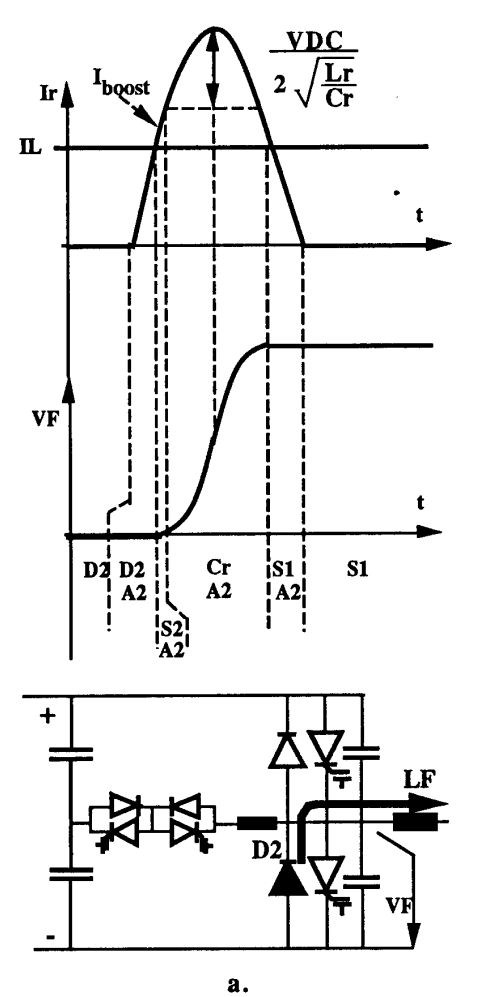
\includegraphics[width=\textwidth]{P1_Fig7a_state1_D2_conducting}
  \caption*{\textbf{(a)} $D_2$ conducts\\$\vf=0,\ \ir=0$}
  \label{fig:P1Fig7a}
\end{subfigure}\hfill
\begin{subfigure}[b]{0.30\textwidth}
  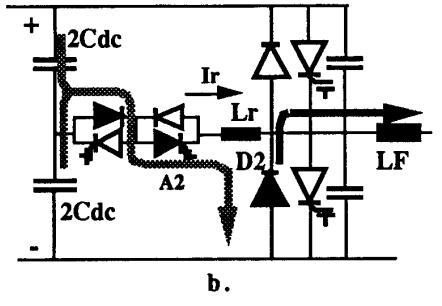
\includegraphics[width=\textwidth]{P1_Fig7b_state2_A1_boost_start}
  \caption*{\textbf{(b)} $A_1$ fires\\$\ir$ ramps up}
  \label{fig:P1Fig7b}
\end{subfigure}\hfill
\begin{subfigure}[b]{0.30\textwidth}
  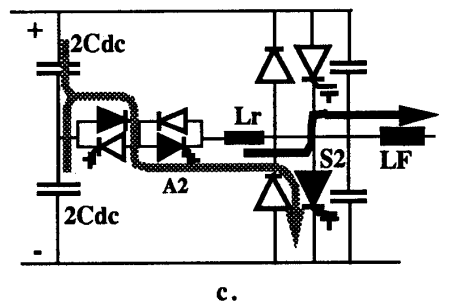
\includegraphics[width=\textwidth]{P1_Fig7c_state3_boost_complete}
  \caption*{\textbf{(c)} Boost complete\\swing begins}
  \label{fig:P1Fig7c}
\end{subfigure}
\\[0.8em]
% Row 2
\begin{subfigure}[b]{0.30\textwidth}
  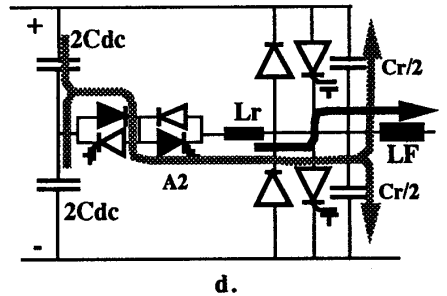
\includegraphics[width=\textwidth]{P1_Fig7d_state4_resonant_swing}
  \caption*{\textbf{(d)} LC resonant\\swing ($\vf \to \Vdc$)}
  \label{fig:P1Fig7d}
\end{subfigure}\hfill
\begin{subfigure}[b]{0.30\textwidth}
  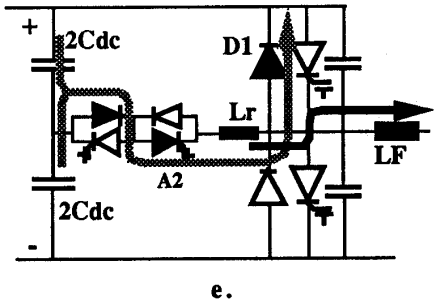
\includegraphics[width=\textwidth]{P1_Fig7e_state5_upper_diode_clamp}
  \caption*{\textbf{(e)} $D_1$ clamps\\$\vf = \Vdc$, ZVS ready}
  \label{fig:P1Fig7e}
\end{subfigure}\hfill
\begin{subfigure}[b]{0.30\textwidth}
  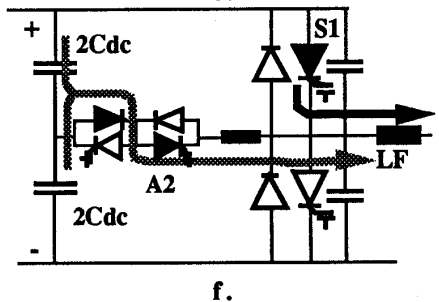
\includegraphics[width=\textwidth]{P1_Fig7f_state6_ir_ramps_down}
  \caption*{\textbf{(f)} $\ir \to 0$\\$S_1$ fires at ZVS}
  \label{fig:P1Fig7f}
\end{subfigure}
\\[0.8em]
% Row 3 (final state, centred)
\begin{subfigure}[b]{0.30\textwidth}
  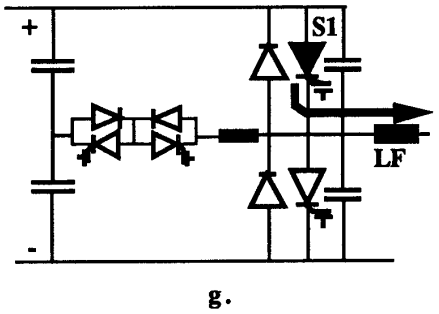
\includegraphics[width=\textwidth]{P1_Fig7g_state7_S1_steady}
  \caption*{\textbf{(g)} $S_1$ conducts\\$\ir=0$, steady state}
  \label{fig:P1Fig7g}
\end{subfigure}
\caption{P1 Fig.\,7 — Commutation from Diode: seven switching states (a)--(g).
         Source: De Doncker \& Lyons, IEEE IAS 1990, p.\,4--5.}
\label{fig:P1Fig7_all}
\end{figure}

\begin{circuitbox}[State-by-State Circuit Description — P1 Fig.\,7a–g]
\renewcommand{\arraystretch}{1.35}
\begin{tabular}{p{0.6cm} p{2.8cm} p{3.5cm} p{5.0cm}}
\toprule
\textbf{State} & \textbf{Active devices} & \textbf{Pole voltage $\vf$} & \textbf{Inductor current $\ir$} \\
\midrule
(a) & $D_2$ conducts        & $\vf = 0$ (clamped to lower rail)  & $\ir = 0$; no current in aux.\ branch \\
(b) & $A_1$ ON, $D_2$       & $\vf = 0$ (still clamped)          & $\ir$ ramps up linearly: $\dot{\ir} = \Vdc/2\Lr$ \\
(c) & $A_1$ ON, $D_2$       & $\vf = 0$                          & $\ir = \IL + i_\text{boost}$; boost ends, $A_1$ off \\
(d) & $\Lr$--$\Cr$ free     & $\vf$ swings $0 \to \Vdc$ sinusoidally & $\ir$ follows LC circle trajectory \\
(e) & $D_1$ clamps          & $\vf = \Vdc$ (clamped to upper rail) & $\ir = I_\text{peak}$; ZVS condition satisfied \\
(f) & $D_1$, $\Lr$          & $\vf = \Vdc$ (clamped)             & $\ir$ ramps back down: $\dot{\ir} = -\Vdc/2\Lr$ \\
(g) & $S_1$ ON              & $\vf = \Vdc$ (steady)              & $\ir = 0$; aux.\ branch fully off \\
\bottomrule
\end{tabular}
\end{circuitbox}

\begin{statebox}
\begin{tabular}{lll}
\toprule
Symbol & Meaning & Value at key instants \\
\midrule
$\vf$            & Pole-node voltage      & $0$ (states a--c) $\to \Vdc$ (states e--g) \\
$\ir$            & Auxiliary current      & $0 \to I_\text{peak} \to 0$ \\
$i_\text{boost}$ & Boost increment        & Control parameter; set by outer loop \\
$I_\text{peak}$  & Peak auxiliary current & Occurs at end of state (d) \\
$T_\text{boost}$ & Boost phase duration   & States (b)--(c) \\
$T_\text{res}$   & Resonant swing duration & State (d) only \\
\bottomrule
\end{tabular}
\end{statebox}

\begin{eqnbox}
\textbf{State (b) — linear boost ramp:}
\begin{equation}
    \ir(t) = \frac{\Vdc}{2\Lr}\,t, \qquad
    T_\text{boost} = \frac{2\Lr\,i_\text{boost}}{\Vdc}
    \label{eq:T_boost}
\end{equation}

\textbf{State (d) — resonant swing (forced LC oscillator):}
\begin{equation}
    \ddot{\vf} + \omegar^2\,\vf = \omegar^2\cdot\frac{\Vdc}{2},
    \qquad \omegar = \frac{1}{\sqrt{\Lr\Cr}},\quad \Zr = \sqrt{\frac{\Lr}{\Cr}}
    \label{eq:swing_ode}
\end{equation}

Solution with initial conditions $\vf(0)=0$, $\ir(0)=\IL+i_\text{boost}$:
\begin{align}
    \vf(t)  &= \frac{\Vdc}{2}(1 - \cos\omegar t)
               + (\ir(0)-\IL)\,\Zr\sin\omegar t
    \label{eq:vf_swing} \\[4pt]
    \ir(t)  &= \IL + (\ir(0)-\IL)\cos\omegar t
               + \frac{\Vdc/2}{\Zr}\sin\omegar t
    \label{eq:ir_swing}
\end{align}

\textbf{Peak current} (at end of state d, when $\vf = \Vdc$):
\begin{equation}
    I_\text{peak} = \IL + i_\text{boost} + \frac{\Vdc}{2\Zr}
    \label{eq:Ipeak_diode}
\end{equation}

\textbf{Resonant half-swing duration} (state d):
\begin{equation}
    T_\text{res} = \frac{\pi}{\omegar} = \pi\sqrt{\Lr\Cr}
    \label{eq:T_res}
\end{equation}

\textbf{Total commutation time} (states b through f):
\begin{equation}
    T_c = T_\text{boost} + T_\text{res}
        = \frac{2\Lr\,i_\text{boost}}{\Vdc} + \pi\sqrt{\Lr\Cr}
    \label{eq:T_comm_diode}
\end{equation}
\end{eqnbox}

\begin{physbox}
\textbf{Why seven states?} Each state has a distinct set of conducting devices,
so the governing equation changes at each transition.

\textbf{States (a)--(c)} are purely inductive: $\vf$ is pinned to 0 by $D_2$,
so the full $\Vdc/2$ appears across $\Lr$ and drives a linear current ramp.
This is energy storage, not switching.

\textbf{State (d)} is the only state where the LC oscillator is active.
The circular trajectory in the $(\vf,\, \ir-\IL)$ phase plane must reach
$\vf = \Vdc$ for ZVS.  Circle radius:
$R = \sqrt{i_\text{boost}^2 + (\Vdc/2\Zr)^2}$.
ZVS is satisfied when $i_\text{boost} \geq 0$.

\textbf{State (f)} recovers residual energy from $\Lr$ back into the DC bus
through $D_1$ — this is why the auxiliary circuit is lossless in the ideal case.

\textbf{State (g)} is the new idle state. The sequence (a)$\to$(g) is the
complete low-to-high transition; the symmetric high-to-low uses $A_2$ instead
of $A_1$ and is the mirror image.
\end{physbox}

% ============================================================
\section{Master Figure Reference Table}
% ============================================================

\begin{longtable}{p{5.8cm} p{1.0cm} p{1.5cm} p{5.0cm}}
\toprule
\textbf{Filename (omit \texttt{.png})} & \textbf{Pg} & \textbf{Section} & \textbf{Key Equation(s)} \\
\midrule
\endhead
\texttt{P1\_Fig5\_ARCP\_pole\_leg}              & 3    & \ref{sec:P1Fig5}  & \eqref{eq:dvf_dt}--\eqref{eq:shifted_states} \\
\midrule
\texttt{P1\_Fig7a\_state1\_D2\_conducting}      & 4    & \ref{sec:P1Fig7}  & — \\
\texttt{P1\_Fig7b\_state2\_A1\_boost\_start}    & 4    & \ref{sec:P1Fig7}  & \eqref{eq:T_boost} \\
\texttt{P1\_Fig7c\_state3\_boost\_complete}     & 4    & \ref{sec:P1Fig7}  & \eqref{eq:T_boost} \\
\texttt{P1\_Fig7d\_state4\_resonant\_swing}     & 4--5 & \ref{sec:P1Fig7}  & \eqref{eq:swing_ode}--\eqref{eq:ir_swing} \\
\texttt{P1\_Fig7e\_state5\_upper\_diode\_clamp} & 5    & \ref{sec:P1Fig7}  & \eqref{eq:Ipeak_diode} \\
\texttt{P1\_Fig7f\_state6\_ir\_ramps\_down}     & 5    & \ref{sec:P1Fig7}  & \eqref{eq:T_comm_diode} \\
\texttt{P1\_Fig7g\_state7\_S1\_steady}          & 5    & \ref{sec:P1Fig7}  & — \\
\bottomrule
\caption{Currently available figures (8 PNGs). Add rows as new figures are extracted.}
\label{tab:master_index}
\end{longtable}

\end{document}
